\documentclass[11pt,a4paper]{article}

\usepackage[a4paper,top=22mm,bottom=22mm,left=24mm,right=22mm]{geometry}
\usepackage{fontspec}
\usepackage{xcolor}
\usepackage{graphicx}
\usepackage{booktabs}
\usepackage{tabularx}
\usepackage{array}
\usepackage{enumitem}
\usepackage{titlesec}
\usepackage{fancyhdr}
\usepackage{hyperref}
\usepackage{caption}
\usepackage{float}
\usepackage{amsmath}

\defaultfontfeatures{Ligatures=TeX}
\setmainfont{Times New Roman}
\setsansfont{Arial}
\setmonofont{Consolas}

\definecolor{graphite}{HTML}{292D32}
\definecolor{warmorange}{HTML}{D46632}
\definecolor{sand}{HTML}{F3EEE6}
\definecolor{softgray}{HTML}{F4F5F6}
\definecolor{linegray}{HTML}{CBD0D5}
\definecolor{linkblue}{HTML}{315D7C}

\hypersetup{colorlinks=true,linkcolor=graphite,urlcolor=linkblue,citecolor=linkblue,pdfauthor={Zihan Wang},pdftitle={Experiment 3 Desktop Object Automatic Classification and Sorting}}
\setlength{\parindent}{0pt}
\setlength{\parskip}{5pt}
\setlength{\headheight}{22pt}
\setlist[itemize]{leftmargin=6mm,itemsep=2pt,topsep=3pt}
\captionsetup{font=small,labelfont={bf,color=warmorange}}

\titleformat{\section}{\sffamily\Large\bfseries\color{graphite}}{\color{warmorange}\thesection}{0.7em}{}[\vspace{2pt}\color{warmorange}\titlerule]
\titleformat{\subsection}{\sffamily\large\bfseries\color{graphite}}{\thesubsection}{0.6em}{}

\pagestyle{fancy}
\fancyhf{}
\fancyhead[L]{\sffamily\small Zihan Wang \textbar{} Robotics Integration Group Project I}
\fancyhead[R]{\sffamily\small Experiment 3 Desktop Sorting Simulation}
\fancyfoot[L]{\sffamily\footnotesize Individual experiment report}
\fancyfoot[R]{\sffamily\footnotesize Page \thepage}
\renewcommand{\headrulewidth}{0.4pt}
\renewcommand{\headrule}{\hbox to\headwidth{\color{linegray}\leaders\hrule height \headrulewidth\hfill}}

\newcommand{\metric}[2]{\begin{minipage}[t]{0.22\textwidth}\colorbox{softgray}{\parbox[c][17mm][c]{0.93\linewidth}{\centering\sffamily\bfseries\color{warmorange}\Large #1\\[-1pt]\normalfont\small\color{graphite}#2}}\end{minipage}}

\begin{document}

\begin{titlepage}
\vspace*{25mm}
\noindent\colorbox{graphite}{\rule{13mm}{0pt}\rule[-155mm]{0pt}{190mm}}\hspace{3mm}%
\colorbox{warmorange}{\rule{2mm}{0pt}\rule[-155mm]{0pt}{190mm}}\hspace{8mm}%
\begin{minipage}[t]{0.72\textwidth}\raggedright
{\sffamily\color{warmorange}\bfseries\Large ROBOTICS INTEGRATION GROUP PROJECT I}\par
\vspace{7mm}
{\sffamily\bfseries\fontsize{23}{28}\selectfont\color{graphite}Experiment 3\\[2mm]Desktop Object Automatic\\Classification and Sorting}\par
\vspace{5mm}
{\sffamily\Large\color{graphite}ROS 2, Gazebo and MoveIt simulation}\par

\vspace{18mm}
\colorbox{sand}{\parbox{0.92\linewidth}{\vspace{5mm}\begin{tabular}{@{}>{\sffamily\bfseries}p{33mm}p{67mm}@{}}
Student & Zihan Wang \\
Student ID & 24020036065 \\
Personal role & Simulation integration and motion-flow collaboration \\
Task classes & 0: green original; 1: yellow pineapple \\
Runtime & ROS 2 Humble, Gazebo, MoveIt 2 \\
Report date & 27 September 2026 \\
\end{tabular}\vspace{5mm}}}

\vfill
{\sffamily\small\color{graphite}This individual report is based on the E3 simulation source code, configuration, launch files, workflow record, screenshots and demonstration material supplied with the project.}
\end{minipage}
\end{titlepage}

\tableofcontents
\clearpage

\section{Basic Requirements of the Experiment}

The objective of Experiment 3 is to build an autonomous desktop-object sorting system. The system must acquire an overhead RGB image, detect objects, map each detection to a fixed desktop grid, command a robot to pick the object, and place it in the correct classification area. For this task, the two semantic classes are \textbf{original-flavor green milk cartons (class 0)} and \textbf{pineapple-flavor yellow milk cartons (class 1)}.

The simulation design addresses the following requirements:
\begin{itemize}
  \item at least two object classes, six fixed pick grids, and two placement bins;
  \item image input through ROS 2 and structured detection messages containing class, bounding box and confidence;
  \item automatic selection of the nearest calibrated grid rather than manual selection of a target;
  \item a feedback-capable ROS 2 Action for serial pick-and-sort execution;
  \item no manual class, grid or placement decision after the task begins;
  \item collision-aware motion planning, a safe clearance pose, and controlled gripper attachment/detachment;
  \item handling of missing or unstable detections, motion-planning failures, attachment timeouts and uncertain object state;
  \item one launch command that starts the simulator, planning stack, detector, action server and task manager.
\end{itemize}

The supplied project implements a fixed-workspace solution. It uses calibrated grid centers and pre-validated joint configurations, which is appropriate for repeatable desktop sorting and avoids requiring arbitrary pose grasping.

\section{Personal Division of Work}

I, \textbf{Zihan Wang}, was responsible for \textbf{simulation integration and motion-flow collaboration}. My work focused on connecting the perception, grid-assignment, task-queue and robot-execution modules into one serial process. The key contributions were:
\begin{itemize}
  \item checking the interface from visual detections to the task manager, including confidence filtering, class validation and nearest-grid assignment;
  \item participating in the design of the stable observation stage, where a complete six-grid result must remain consistent over consecutive frames before a queue is frozen;
  \item coordinating the action-level execution sequence: approach, local centering, gripper close, attachment confirmation, fixed lift, common clearance, bin placement, release and safe retreat;
  \item checking the coordination between MoveIt planning, trajectory controllers, grid-specific joint poses and the left/center/right bin slots;
  \item enforcing serial execution: only one object may be handled at a time, and a failed action halts the round instead of advancing the queue;
  \item documenting simulation issues and the corresponding safety-oriented solutions for subsequent RoboMaster EP deployment reference.
\end{itemize}

The detection-model training, real-robot data collection, calibration and deployment were completed by other group members. This report therefore concentrates on the simulation integration work and does not claim individual ownership of those parts.

\section{Implementation Principles}

\subsection{System architecture and one-command startup}

The complete simulation stack is started from the ROS 2 workspace after sourcing the Humble installation and the local overlay. The command used for the supplied project is shown in Figure~\ref{fig:command}.

\begin{figure}[H]
\centering
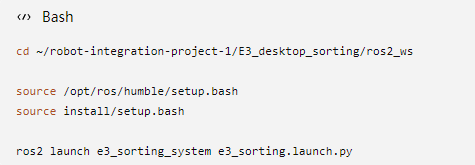
\includegraphics[width=0.68\textwidth]{assets/launch_command.png}
\caption{One-command startup of the E3 desktop-sorting system.}
\label{fig:command}
\end{figure}

The top-level launch file includes the Gazebo simulation and the MoveIt \texttt{move\_group} launch, then creates the detector, pick Action server and task-manager nodes. The Action server is configured for simulation time and enables the Gazebo attachment plugin. This organization avoids a fragile multi-terminal workflow and makes the system boundary explicit (Figure~\ref{fig:launch}).

\begin{figure}[H]
\centering
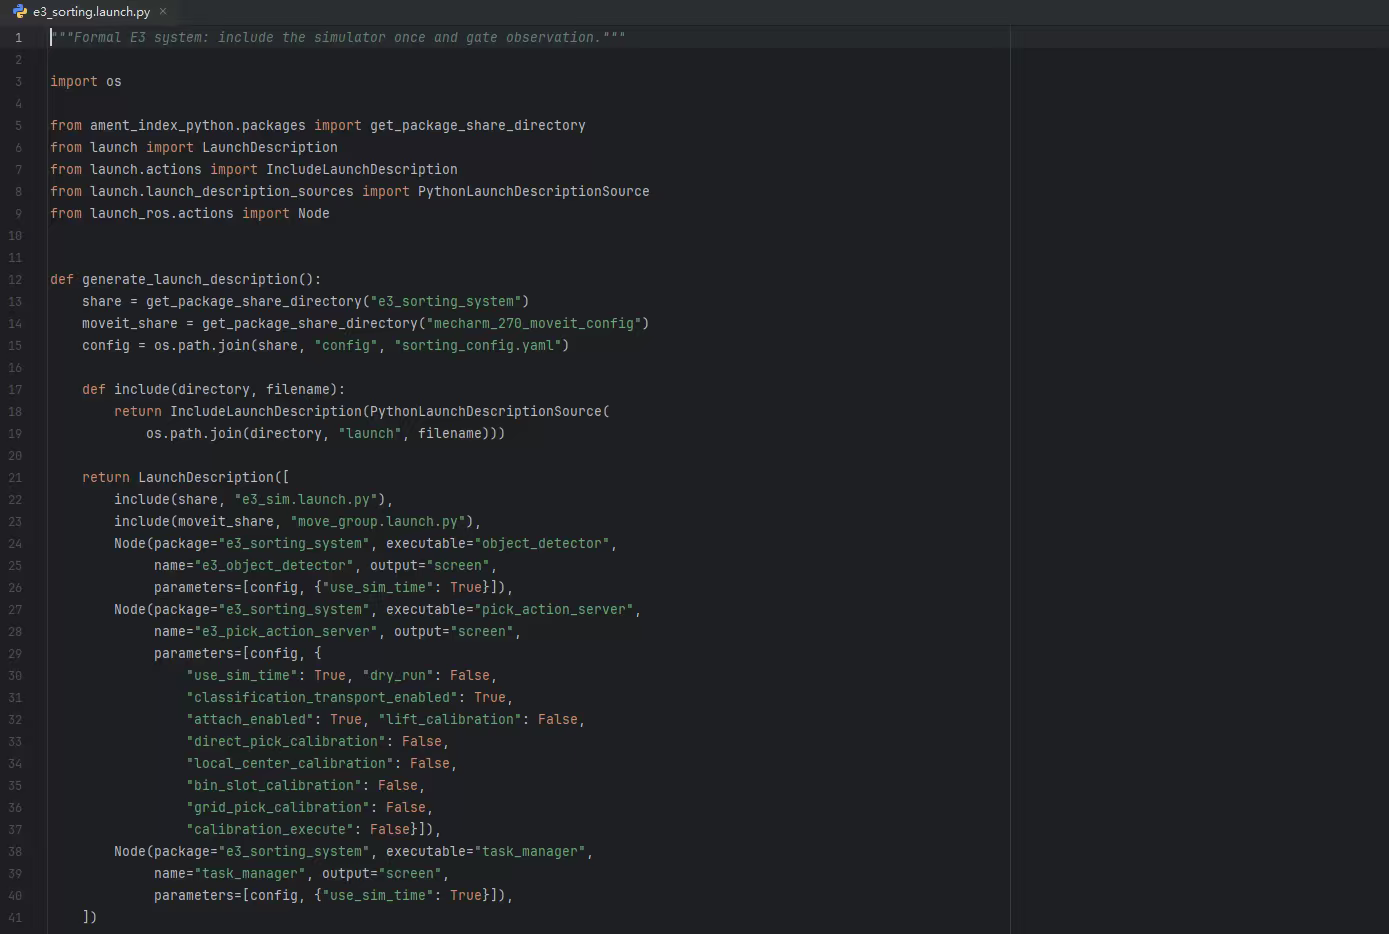
\includegraphics[width=0.94\textwidth]{assets/unified_launch.png}
\caption{Key part of the unified ROS 2 launch file.}
\label{fig:launch}
\end{figure}

The operational data flow is:

\begin{center}
\colorbox{softgray}{\parbox{0.92\textwidth}{\centering
Gazebo overhead camera $\rightarrow$ \texttt{object\_detector} $\rightarrow$ \texttt{/e3/detections} $\rightarrow$ \texttt{task\_manager} $\rightarrow$ \texttt{/e3/pick\_and\_sort} Action $\rightarrow$ \texttt{pick\_action\_server} $\rightarrow$ MoveIt and joint-trajectory controllers}}
\end{center}

\subsection{Perception, filtering and grid assignment}

Each detected box contains a category hypothesis, confidence and center position. The task manager first selects the highest-scoring hypothesis, then rejects invalid numerical values, unsupported categories and scores below the configured confidence threshold. A detection is assigned to the calibrated grid whose pixel center has the smallest Euclidean distance:

\begin{equation}
d_i = \sqrt{(u-u_i)^2 + (v-v_i)^2}.
\end{equation}

The detection is accepted only when the closest distance is within the assignment limit, and when its category is consistent with the expected class for that grid. The code excerpt in Figure~\ref{fig:taskmanager} records the three important decisions: filtering, nearest-grid matching and queue freezing after stable observations.

\begin{figure}[H]
\centering
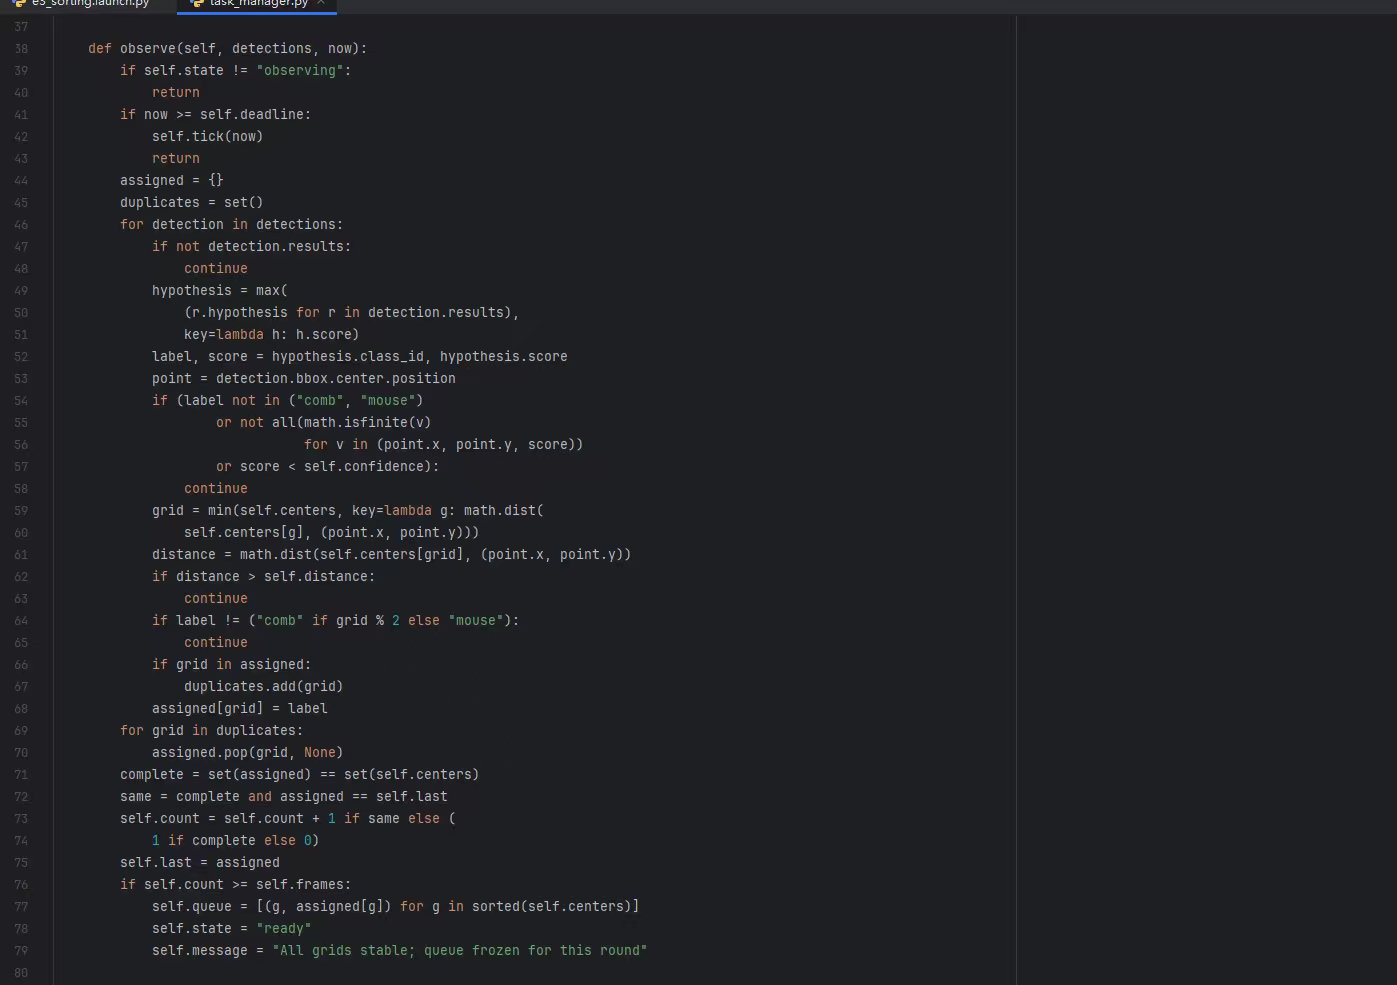
\includegraphics[width=0.94\textwidth]{assets/task_manager_logic.png}
\caption{Task-manager logic for detection filtering, nearest-grid matching and stable-queue freezing. The legacy internal label strings are implementation details; this report uses the milk-carton class definitions stated on the title page.}
\label{fig:taskmanager}
\end{figure}

The configuration requires a minimum confidence of 0.70, a maximum assignment distance of 45 pixels and three consecutive stable frames. These checks prevent one weak or shifted detection from triggering a physical motion.

\subsection{Queue scheduling and ROS 2 Action}

After all six calibrated grids are present and stable, the task manager freezes a queue ordered by grid identifier. It sends one \texttt{PickAndSort} goal at a time, containing the grid identifier, object class and simulation model identifier. The next goal is sent only after the current Action returns success. If a goal is rejected, cancelled or fails, the remaining queue is not executed.

This policy is intentionally conservative. It protects against a common failure mode in automation: treating a failed grasp as if the object had been moved and then continuing with an incorrect scene model.

\subsection{Motion sequence and bin allocation}

The six grids have separate pick and lift joint configurations. After a successful grasp, the robot follows a grid-specific lift configuration, a common high-clearance configuration, an approach configuration for the destination bin, and a left/center/right release configuration. Green original-flavor cartons are routed to the green-class bin, while yellow pineapple-flavor cartons are routed to the yellow-class bin. The column position determines the release slot.

For each object, the sequence is:

\begin{center}
\colorbox{softgray}{\parbox{0.92\textwidth}{\centering
Open gripper $\rightarrow$ fixed pick pose $\rightarrow$ local centering correction $\rightarrow$ close gripper $\rightarrow$ attach/check $\rightarrow$ fixed lift $\rightarrow$ common clearance $\rightarrow$ bin approach $\rightarrow$ slot release $\rightarrow$ detach/open gripper $\rightarrow$ safe retreat}}
\end{center}

Gazebo attachment services are used because gripper friction alone does not reliably hold the simulated cartons. Attachment is accepted only after the gripper has closed and the object is sufficiently close to the grasp link. The process is therefore coupled with follow checks before transporting an object.

\section{Problems Encountered and Solutions}

\begin{table}[H]
\centering
\small
\begin{tabularx}{\textwidth}{@{}>{\bfseries}p{33mm}X X@{}}
\toprule
Problem & Analysis and individual reasoning & Solution adopted \\
\midrule
Repeated inverse-kinematics failure during segmented lifting & Small Cartesian lift increments required fresh IK solutions. Some positions were close to singular or unreachable configurations, so failure probability accumulated across segments. & Replaced long online segmented lifting with calibrated, grid-specific \texttt{lift\_joints}. MoveIt still validates the goal and plans the trajectory; local IK is retained only for millimetre-scale centering correction. \\
Camera occlusion by the arm & In the default pose, the arm blocked the middle grids and only four targets could be observed. Starting the queue from incomplete evidence would produce a false scene model. & Added a controlled observation pose before detection. The manager waits for six stable grid assignments before freezing the queue. \\
Gazebo attachment timeout & Attachment plug-in or simulation-clock stalls can leave the object state uncertain. Blind retrying could produce duplicate constraints or move a detached object. & The Action records the failed stage, stops the round and enters a recovery-required state. It does not advance to the next grid under uncertainty. \\
Objects disturbed during transport & A low route after grasping could pass close to unprocessed objects. & Raised the common clearance configuration and used a fixed safe retreat after release. \\
Queue progression after a failed grasp & Continuing after a failure would make later placement decisions unreliable and hide the failed grid. & Enforced serial execution and stop-on-failure semantics; only a confirmed successful Action allows the next goal. \\
\bottomrule
\end{tabularx}
\caption{Simulation issues and the safety-oriented solutions.}
\label{tab:problems}
\end{table}

The recorded test history includes an attachment timeout at grid 6. The key result is not that a timeout disappeared, but that the system did not continue with an uncertain object state. The earlier grids had completed serial handling before the protected stop. This behavior is aligned with the experiment requirement for exception handling and safe termination.

\section{Verification Evidence and Result}

The supplied project includes the Gazebo world, six grid definitions, two bins, an overhead camera, ROS 2 interfaces, the pick-and-sort Action, configuration files, unit tests and a formal launch file. The detector screenshot in Figure~\ref{fig:detection} is retained as visual evidence of the image-recognition stage.

\begin{figure}[H]
\centering
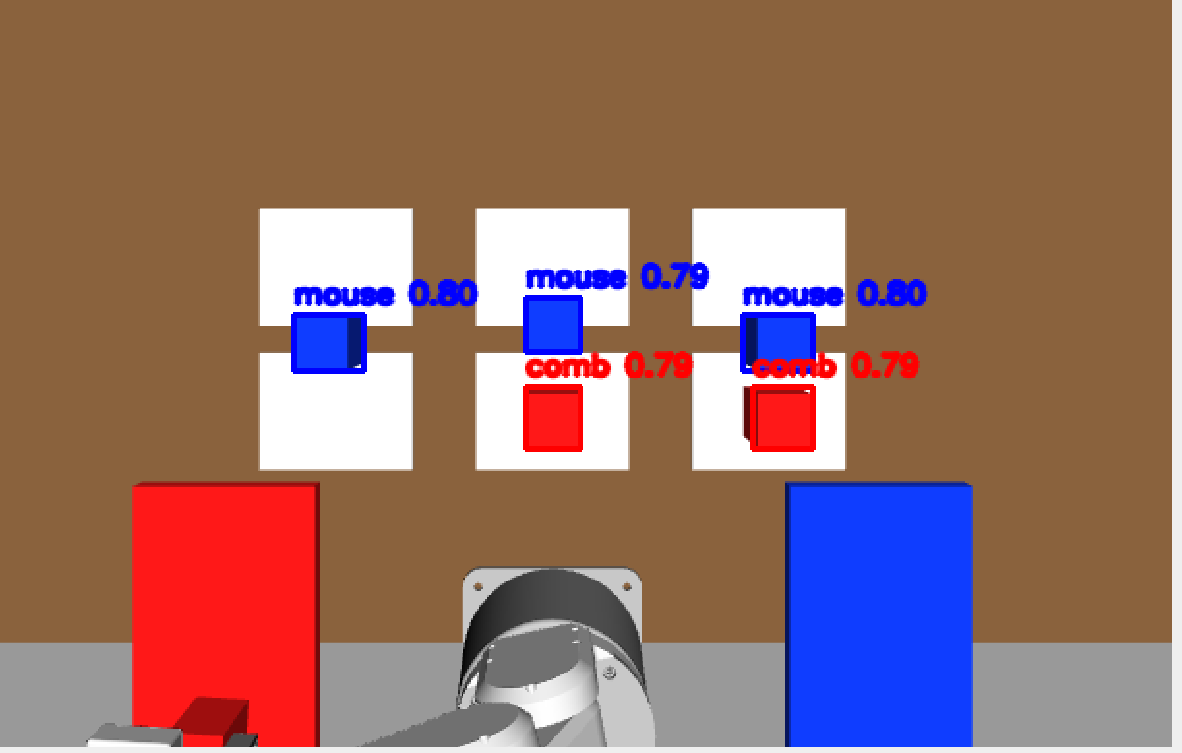
\includegraphics[width=0.74\textwidth]{assets/detection.png}
\caption{Saved detector-stage evidence from the E3 simulation package.}
\label{fig:detection}
\end{figure}

The implementation meets the intended design of two-class fixed-grid sorting, automatic queue construction, serial Action execution and safe failure handling. The available evidence should be described precisely: a complete six-object uninterrupted recording must be verified again before making a stronger claim than the recorded five completed grids followed by a safe stop at the sixth attachment timeout.

\section{Personal Repository and Commit Traceability}

The complete code, report source, screenshots and relevant exercises will be uploaded to my personal repository:

\begin{center}
\url{https://github.com/HesterWang0419/E3-desktop-sorting}
\end{center}

The repository is organized as meaningful development stages rather than one bulk upload:
\begin{enumerate}
  \item add the ROS 2 interfaces, simulation world and initial system structure;
  \item add perception-to-grid scheduling and stable queue management;
  \item add fixed-lift motion, bin-slot routes and failure safeguards;
  \item add launch instructions, tests and workflow documentation;
  \item add this English individual report and the commit-history evidence.
\end{enumerate}

\begin{figure}[H]
\centering
\fbox{\parbox[c][46mm][c]{0.90\textwidth}{\centering\sffamily\color{graphite}Commit-history page screenshot will be inserted here after the repository is pushed.}}
\caption{Reserved location for the required GitHub/Gitee commit-history screenshot.}
\label{fig:commit-history}
\end{figure}

\section{Conclusion}

This project applies ROS 2, Gazebo, MoveIt and a camera-based detector to a fixed-grid desktop sorting task. My simulation contribution was to integrate the perception, assignment, queue and robot-motion stages into a conservative serial workflow. The most important design choice was replacing unstable repeated IK lifting with verified fixed lift configurations, while preserving local correction and MoveIt state validation. Together with stable-frame confirmation, attachment checks, clearance routes and stop-on-failure behavior, the system provides a reproducible simulation basis for the subsequent RoboMaster milk-carton task.

\end{document}
